% !TEX root = arbeit.tex
\appendix
	
\section{Appendix} 
	\subsection{Papers}
	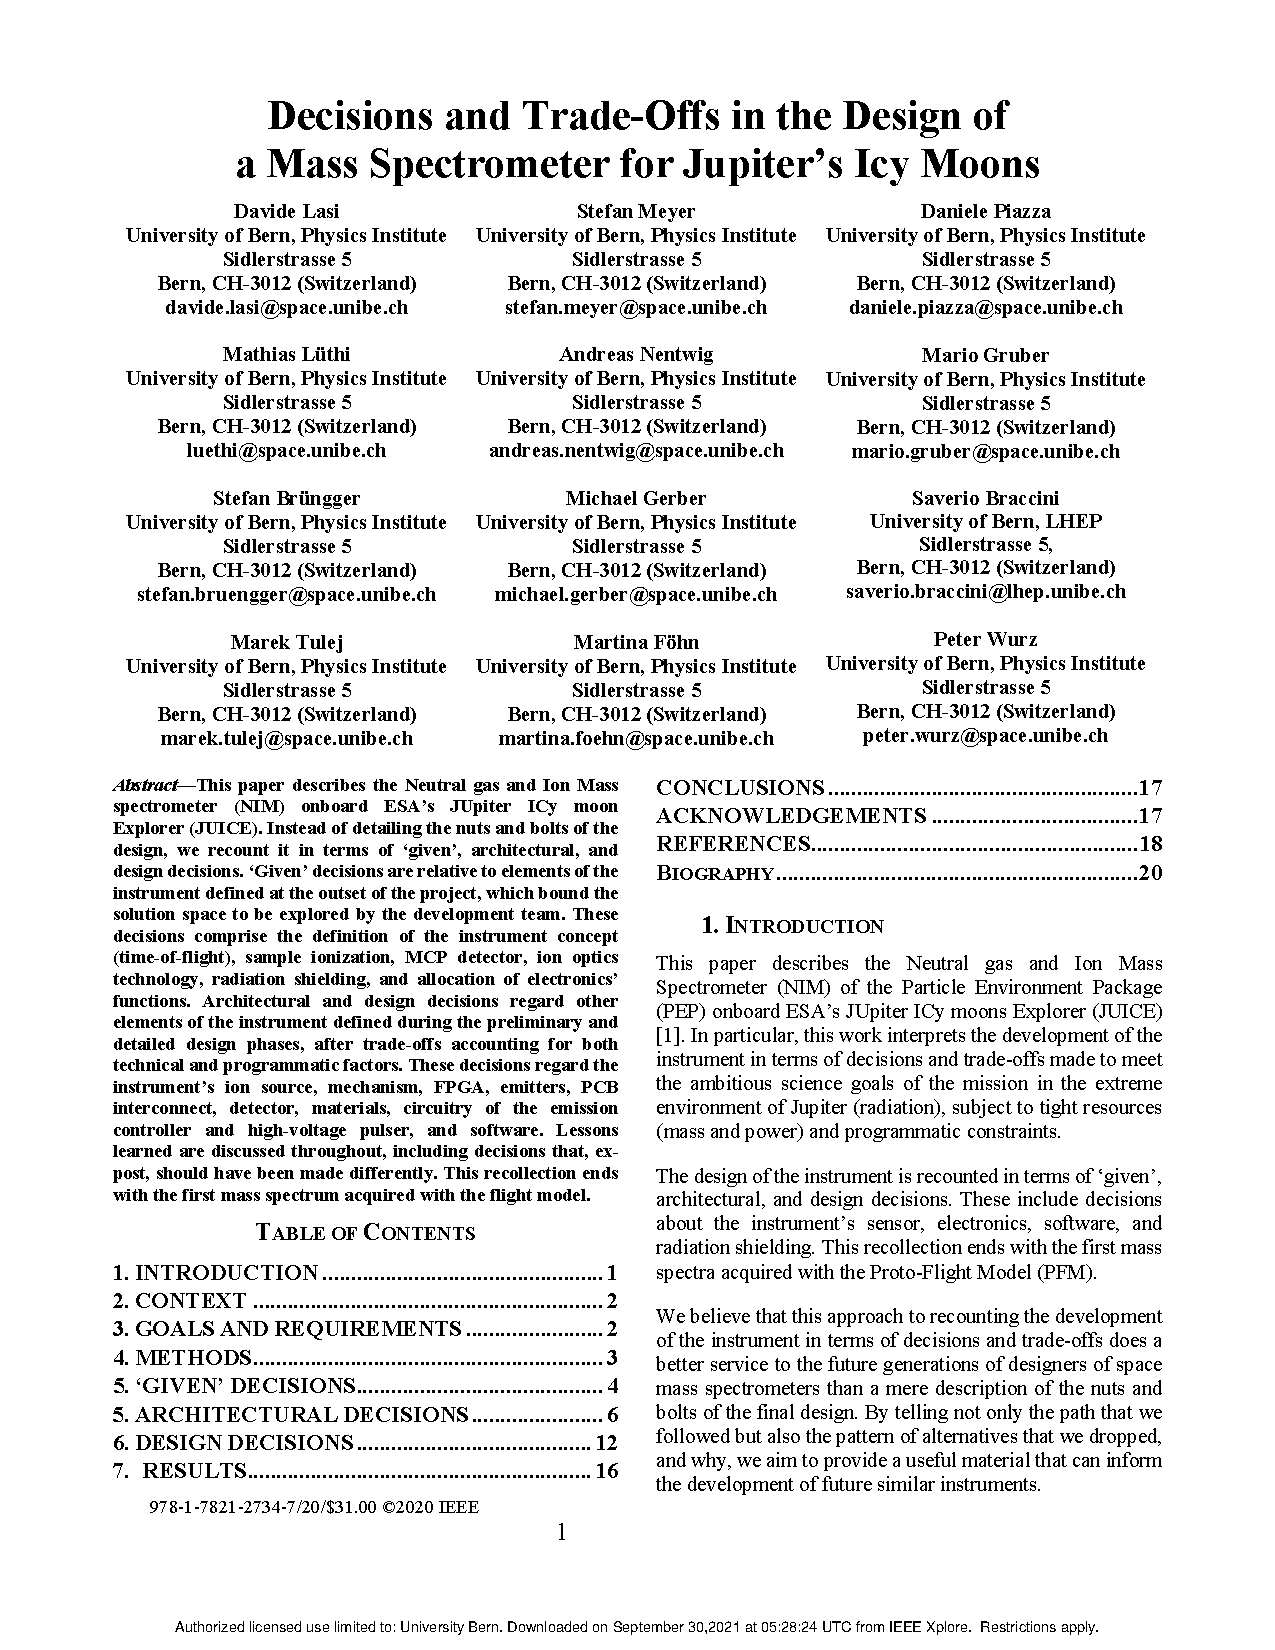
\includepdf[pages={1-}]{Lasi_2020_final.pdf}
	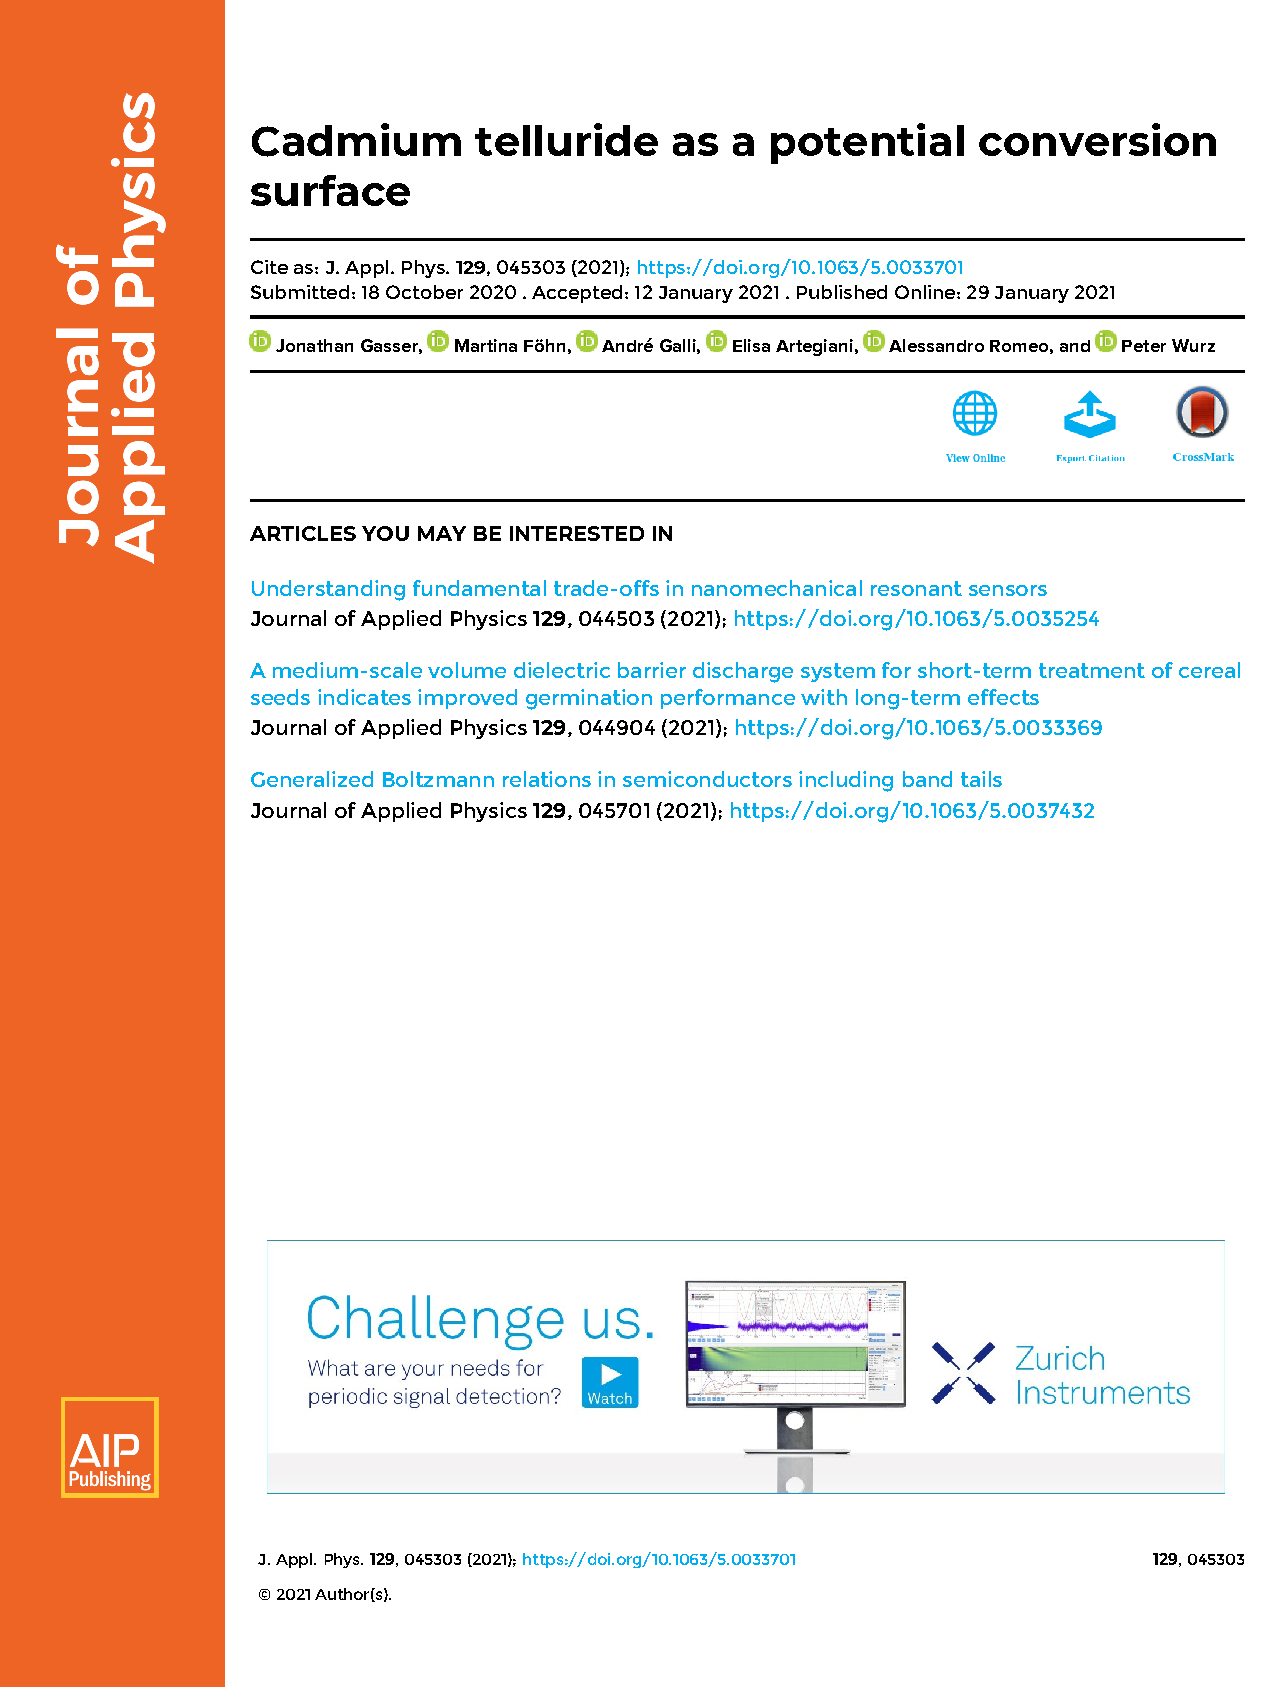
\includepdf[pages={1-}]{Gasser2021_CdTe.pdf}
	
	\subsection{Datasheets} \label{sec:appendix}
	% Filaments. Or put in the true procedure for the filaments and not the unaccurate ones? Would be more useful for an experimenter.
	% MCP Startup procedure
	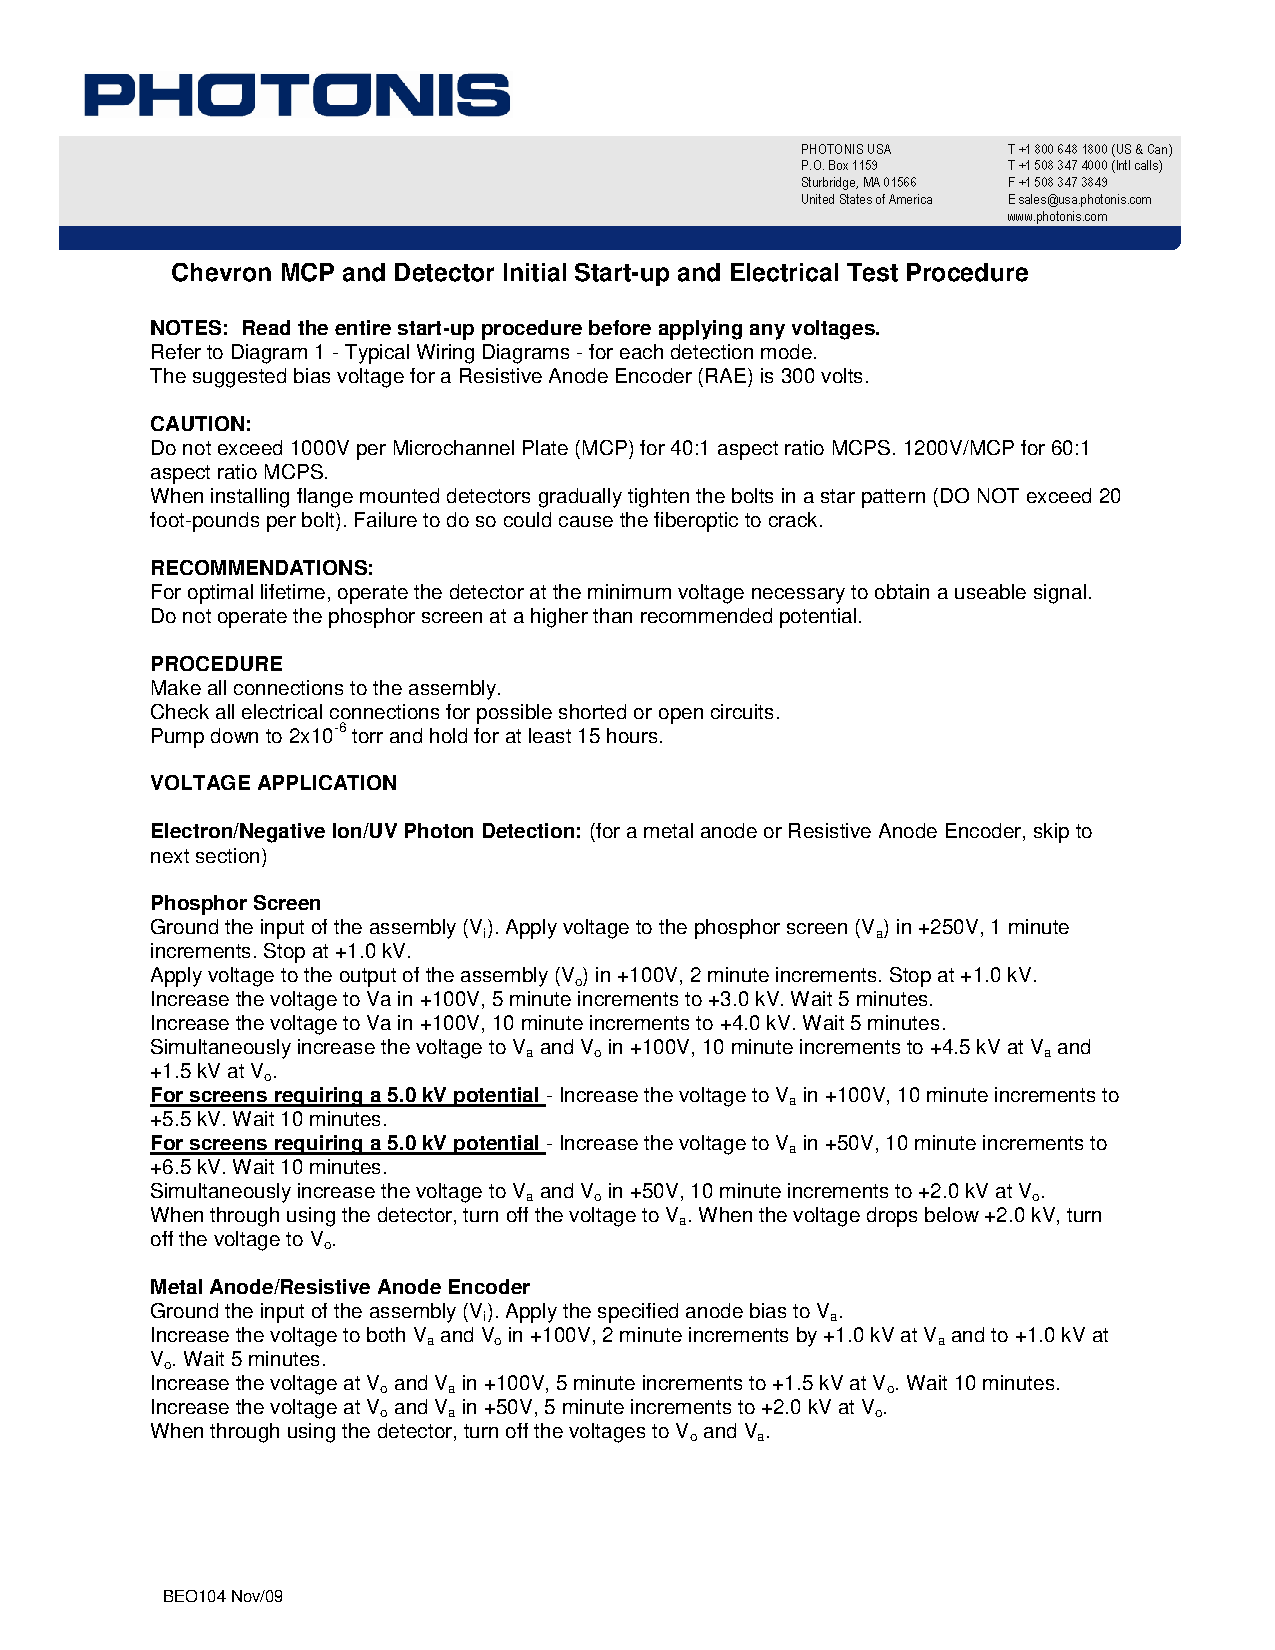
\includepdf[pages=-]{MCP_Startup_procedure.pdf}

